\section{Общие сведения}

\textbf{Вариант:} A-5.\\
\textbf{Объём выборки:} n = 200.\\
\textbf{Единицы измерения:} мс.\\
Данные представлены в виде четырех столбцов \(X_1, X_2, X_3, X_4.\)

\section{Первичное описание выборки}

\subsection{Построение вариационного ряда}

Для каждого столбца строится вариационный ряд $x_{(1)} \le x_{(2)} \le \cdots \le x_{(n)}$. 

\begin{figure}[H]
    \centering
    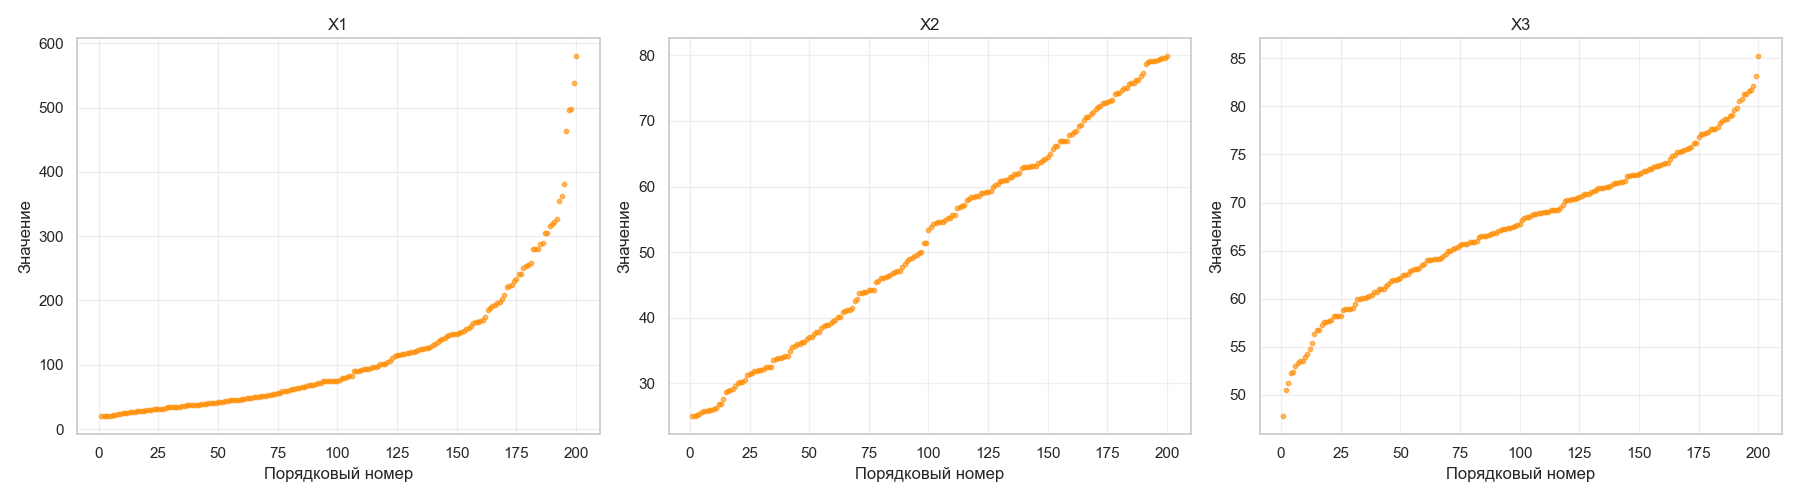
\includegraphics[width=1\linewidth]{pic/plot_2026-04-11 02-52-56_0.png}
    \caption{Вариационный ряд}
    \label{fig:placeholder}
\end{figure}

\subsection{Построение эмпирической функции распределения $F_n(x)$}

Эмпирическая частота $\nu_n(x)$ — число элементов выборки, меньших $x$. 

Эмпирическая функция распределения (ЭФР) определяется как:

$$
F_n(x) = \frac{\nu_n(x)}{n}.
$$

\begin{figure}[H]
    \centering
    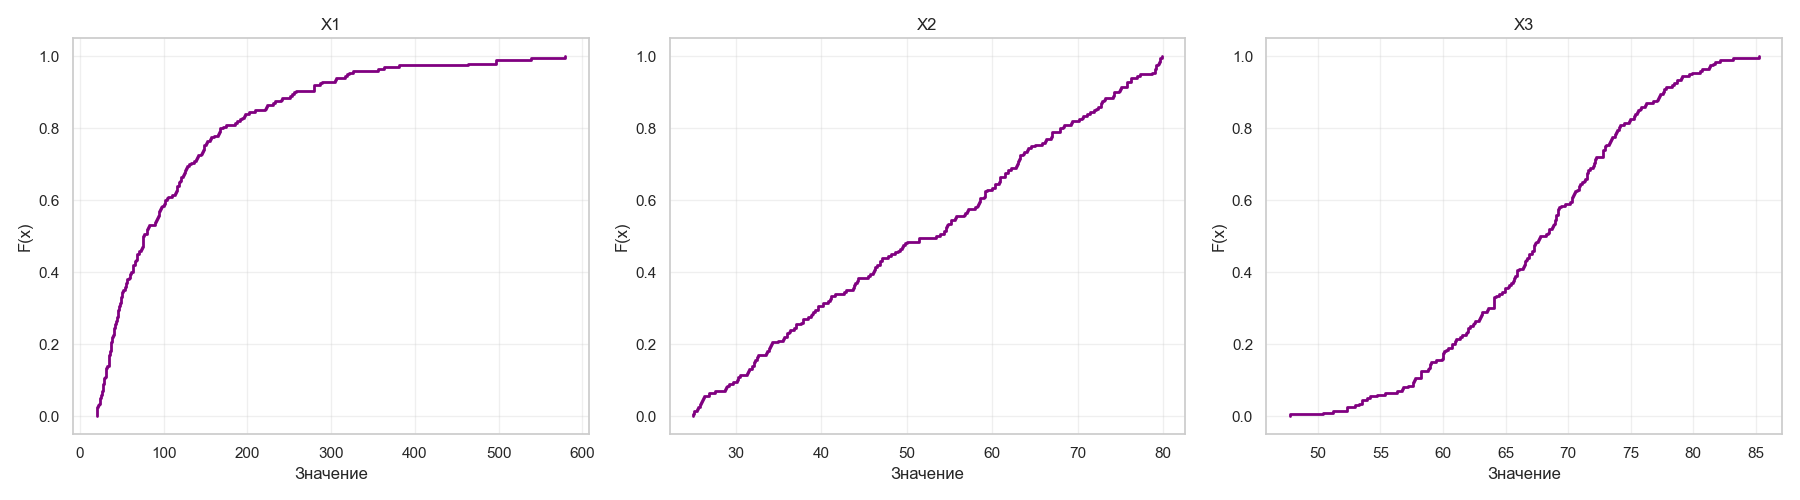
\includegraphics[width=1\linewidth]{pic/plot_2026-04-11 02-52-56_1.png}
    \caption{Эмпирическая функция распределения}
    \label{fig:placeholder}
\end{figure}

\newpage

\subsection{Построение гистограммы и обоснование выбора числа интервалов}

Для анализа формы распределения были построены гистограммы с использованием трёх различных правил:
\begin{itemize}
    \item Правило Стерджеса:  $h = 3.5 \cdot S \cdot n^{-1/3}$.$
    \item Правило Скотта: h = 2 \cdot \mathrm{IQR} \cdot n^{-1/3}$.
    \item Правило Фридмана-Диакониса: $k = 1 + \lfloor \log_2 n \rfloor$.
\end{itemize}

\begin{figure}[H]
    \centering
    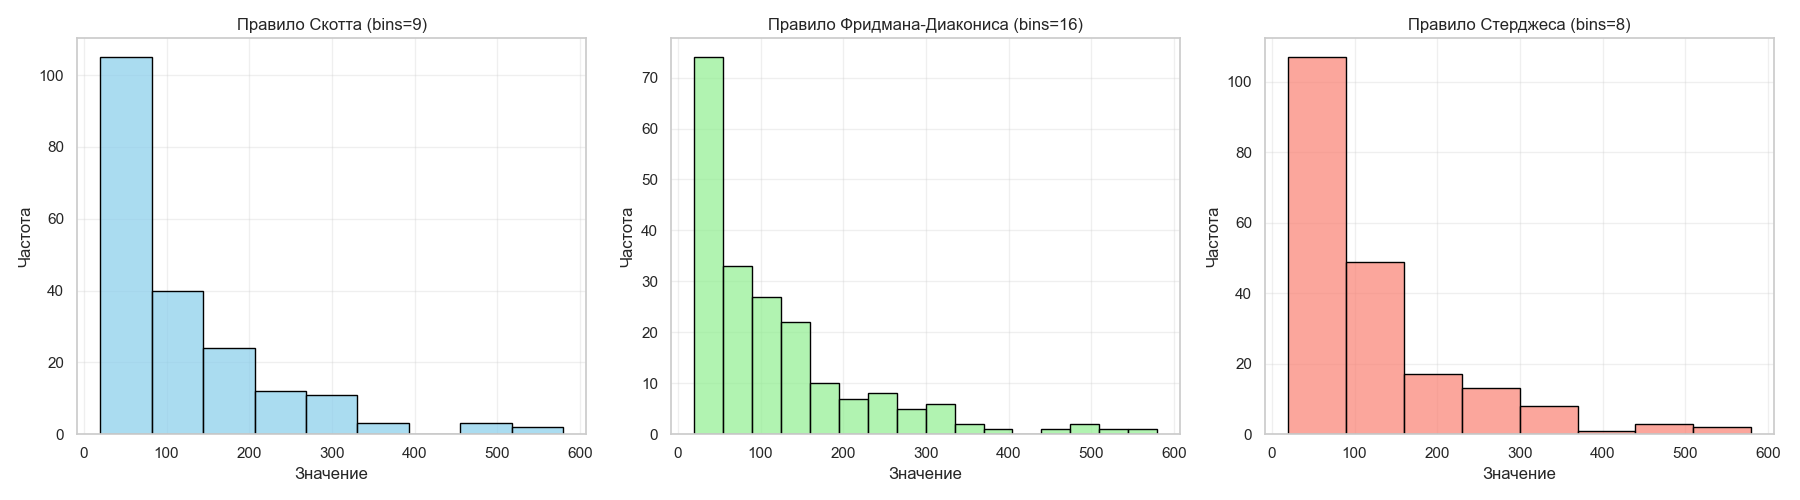
\includegraphics[width=1\linewidth]{pic/plot_2026-04-11 02-52-56_2.png}
    \caption{Сравнение правил разбиения гистограммы для $X_1$}
    \label{fig:placeholder}
\end{figure}

\begin{figure}[H]
    \centering
    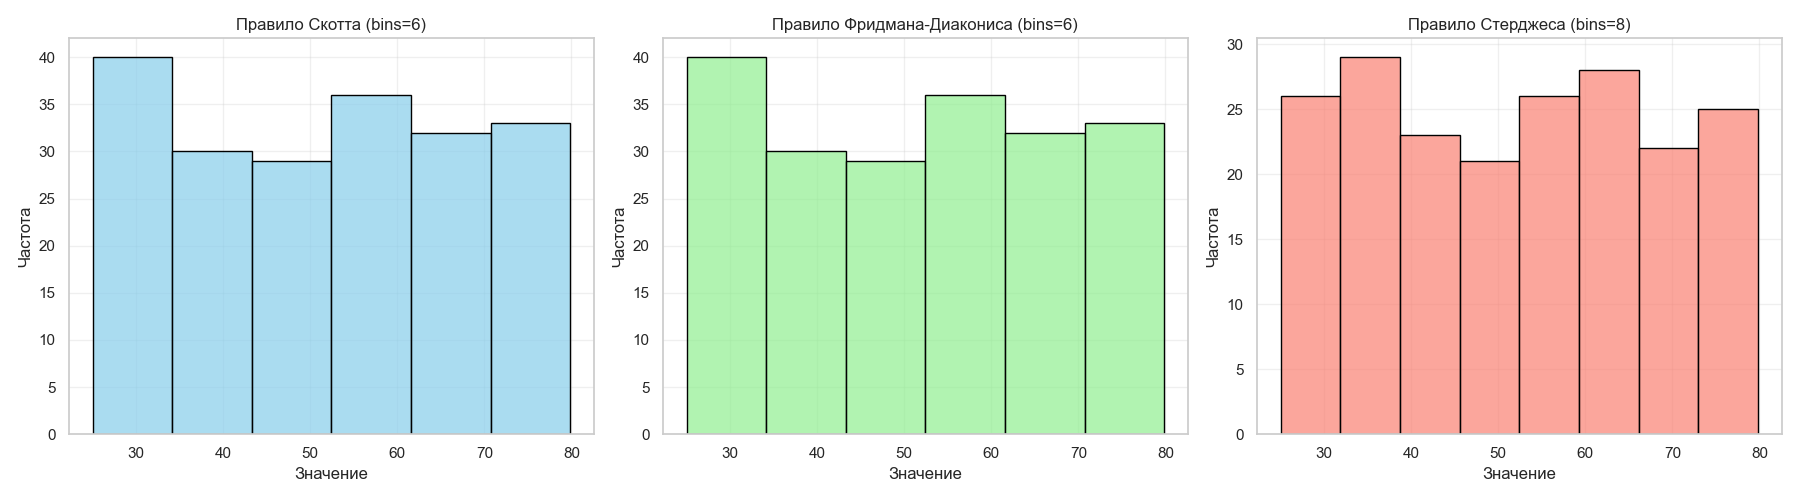
\includegraphics[width=1\linewidth]{pic/plot_2026-04-11 02-52-56_3.png}
    \caption{Сравнение правил разбиения гистограммы для $X_2$}
    \label{fig:placeholder}
\end{figure}

\begin{figure}[H]
    \centering
    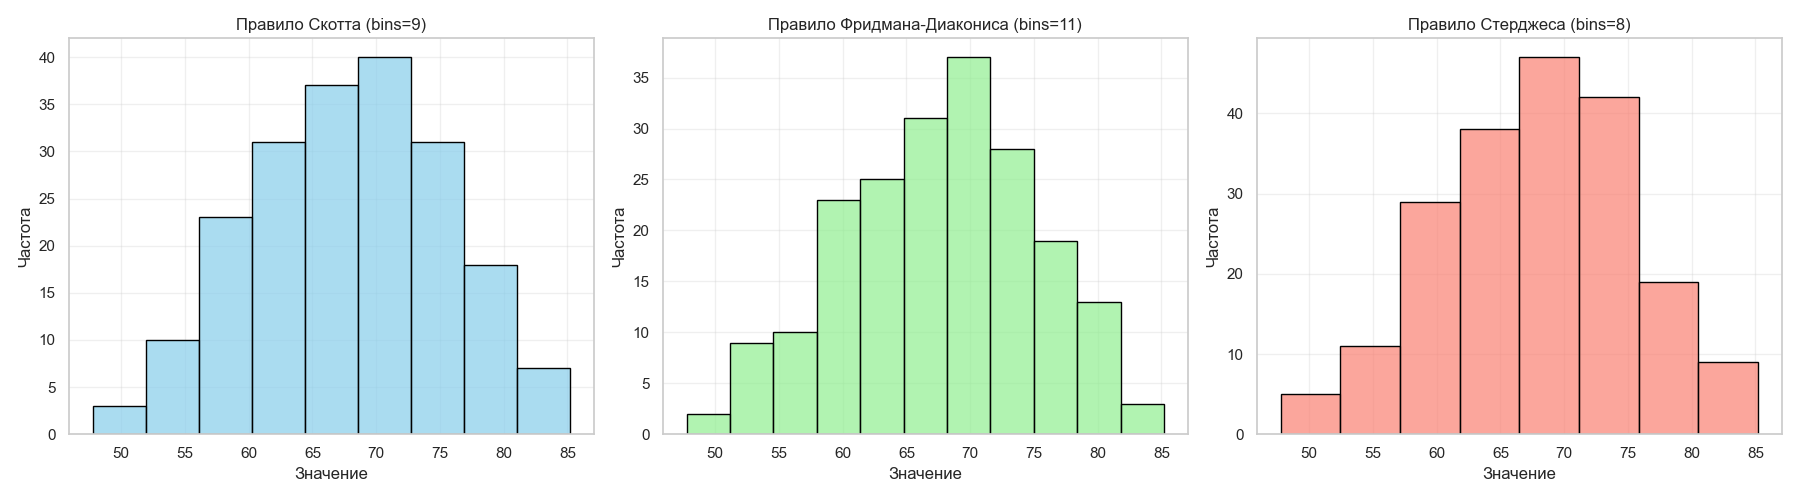
\includegraphics[width=1\linewidth]{pic/plot_2026-04-11 02-52-56_4.png}
    \caption{Сравнение правил разбиения гистограммы для $X_3$}
    \label{fig:placeholder}
\end{figure}

\newpage

\subsection{Вычисление числовых характеристик}

На основе выборки вычислены точные основные показатели:

\begin{table}[htbp]
\centering
\caption{Числовые характеристики выборок X1, X2, X3}
\label{tab:stats}
\begin{tabular}{lccc}
Показатель & X1 & X2 & X3 \\
\midrule
Среднее ($\bar{x}$) & 115.940000 & 51.880000 & 67.700000 \\
Смещ. дисперсия ($S^2$) & 10866.100000 & 266.360000 & 56.570000 \\
Несмещ. дисперсия ($\hat{\sigma}^2$) & 10920.700000 & 267.690000 & 56.850000 \\
Смещ. откл. ($S$) & 104.240000 & 16.320000 & 7.520000 \\
Несмещ. откл. ($\hat{\sigma}$) & 104.500000 & 16.360000 & 7.540000 \\
Медиана ($m_e$) & 75.910000 & 53.630000 & 67.980000 \\
Q1 (25\%) ($Q_1$) & 42.230000 & 37.060000 & 62.360000 \\
Q3 (75\%) ($Q_3$) & 148.270000 & 64.620000 & 72.980000 \\
\bottomrule
\end{tabular}
\end{table}

\section{Предположение о виде закона распределения}

Анализируя графики:
\begin{itemize}
    \item[$X_1$]: Ярко выраженная правосторонняя асимметрия, резкий спад, есть естественная граница слева (около 20). Подходит \textbf{экспоненциальное распределение со сдвигом} $Exp(\lambda, c)$.
    
    \item[$X_2$]: Распределение визуально плоское, ограничено рамками $\approx 25$--$80$, без ярко выраженного центра. Подходит \textbf{равномерное распределение} $U(a,b)$.
    
    \item[$X_3$]: Колоколообразная форма, симметрия относительно центра, среднее ($\approx 66.7$) почти равно медиане ($\approx 66.9$). Подходит \textbf{нормальное распределение} $\mathcal{N}(a, \sigma)$.
\end{itemize}

\section{Оценивание параметров}

Вычислим оценки по Методу Моментов (ММ) и Методу Максимального Правдоподобия (ММП).

\subsection{Экспоненциальное распределение со сдвигом ($X_1 \sim Exp_{\lambda,c}$)}

\textbf{Метод моментов (ММ):} Приравниваем теоретические моменты к выборочным: $EX = c + \frac{1}{\lambda} = \bar{x}$, $DX = \frac{1}{\lambda^2} = S^2$.

$$
\hat{\lambda} = \frac{1}{\sqrt{S^2}} = \frac{1}{104.24} \approx 0.0096, \quad \hat{c} = \bar{x} - \frac{1}{\hat{\lambda}} = 115.94 - 104.24 \approx 11.70
$$

\textbf{Метод максимального правдоподобия (ММП):} Функция правдоподобия:

$$
L(\lambda, c) = \lambda^n e^{-\lambda \sum_{i=1}^{n}(x_i - c)} \prod_{i=1}^{n} I(x_i \ge c)
$$

Оценка сдвига ограничена минимумом выборки, являющимся достаточной статистикой для $c$:

$$
\hat{\lambda} = \frac{1}{\bar{x} - \hat{c}} = \frac{1}{115.94 - 19.97} \approx 0.0104 ,\quad  \hat{c} = x_{(1)} = 19.97, 
$$

\textbf{Сравнение:} Методы дают значительные различия. Оценка параметра сдвига $c$ по ММ ($11.70$) значительно ниже, чем по ММП ($19.97$), с относительной разностью $+70.70\%$. Оценки ММП предпочтительнее, так как они гарантируют, что теоретическая нижняя граница не превысит фактический наблюдаемый минимум выборки.


\subsection{Равномерное распределение ($X_2 \sim U(a, b)$)}

\textbf{Метод моментов (ММ):} Приравниваем теоретические моменты к выборочным: $EX = \frac{a+b}{2} = \bar{x}$, $DX = \frac{(b-a)^2}{12} = S^2$. Решая систему:

$$
\hat{a} = \bar{x} - \sqrt{3S^2} = 51.88 - \sqrt{3 \cdot 266.36} \approx 23.61
$$

$$
\hat{b} = \bar{x} + \sqrt{3S^2} = 51.88 + \sqrt{3 \cdot 266.36} \approx 80.15
$$

\textbf{Метод максимального правдоподобия (ММП):} Функция правдоподобия:

$$
L(a, b) = \frac{1}{(b-a)^n} \prod_{i=1}^{n} I(a \le x_i \le b)
$$

Чтобы максимизировать $L$, знаменатель $(b-a)$ должен быть минимальным при условии, что все $x_i$ лежат внутри $[a, b]$. Отсюда оценки — крайние члены вариационного ряда:

$$
\hat{a} = x_{(1)} = 24.99, \quad \hat{b} = x_{(n)} = 79.85
$$

\textbf{Сравнение:} Наблюдаются заметные различия. ММ занижает нижнюю границу $a$ ($23.61$ против $24.99$) и завышает верхнюю $b$ ($80.15$ против $79.85$), расширяя интервал. ММП использует экстремальные значения выборки, что обеспечивает более точные и логичные оценки для распределения с жёсткими границами.

\subsection{Нормальное распределение ($X_3 \sim N(a, \sigma^2)$)}

\textbf{Метод моментов (ММ):} Приравниваем теоретические моменты к выборочным ($EX = \bar{x}$, $DX = S^2$).

$$
\hat{a} = \bar{x} = 67.70, \quad \hat{\sigma}^2 = S^2 = 56.57
$$

\textbf{Метод максимального правдоподобия (ММП):} Функция правдоподобия имеет вид:

$$
L(a, \sigma^2) = \prod_{i=1}^{n} \frac{1}{\sqrt{2\pi\sigma^2}} \exp\left( -\frac{(x_i - a)^2}{2\sigma^2} \right)
$$

Максимизация логарифмической функции правдоподобия даёт оценки, полностью совпадающие с методом моментов:

$$
\hat{a} = \bar{x} = 67.70, \quad \hat{\sigma}^2 = S^2 = 56.57
$$

\textbf{Сравнение:} Оценки ММ и ММП полностью совпадают. Это свойство нормального распределения, где оба метода дают одинаковые результаты: $\hat{\mu} = \bar{x}$ и $\hat{\sigma}^2 = \frac{1}{n}\sum_{i=1}^{n}(x_i - \bar{x})^2$.

\section{Оценивание параметрической вероятности}

Выберем для каждого столбца порог $x_0 = \bar{x} + \hat{\sigma}$ (одно стандартное отклонение вправо от среднего) и оценим вероятность $P(X > x_0)$. Эмпирическая вероятность рассчитывается как доля наблюдений выборки, строго превышающих порог. Параметрическая вероятность рассчитывается по формуле $1 - F(x_0)$, где $F(x)$ — теоретическая функция распределения с параметрами, найденными по ММП.

\subsection{1. $X_1$ (Экспоненциальное распределение со сдвигом)}

Порог: $x_0 = 115.94 + 104.50 = 220.44$.

\begin{itemize}
    \item \textbf{Теоретическая вероятность:} 
    $$
    P = e^{-\hat{\lambda}(x_0 - \hat{c})} = e^{-0.0104 \cdot (220.44 - 19.97)} \approx 0.1238 \quad (12.38\%).
    $$
    \item \textbf{Эмпирическая вероятность:} доля значений $> 220.44$ в выборке составила $0.1500$ ($15.00\%$).
\end{itemize}

\textbf{Сравнение:} Параметрическая оценка ($12.38\%$) ниже эмпирической ($15.00\%$). Абсолютное различие составляет $0.0262$ (относительное различие около $17.5\%$). Это указывает на то, что модель экспоненциального распределения несколько недооценивает вероятность в хвосте распределения. Возможная причина — наличие в выборке нескольких аномально больших значений, которые плохо описываются экспоненциальной моделью.

\subsection{2. $X_2$ (Равномерное распределение)}

Порог: $x_0 = 51.88 + 16.36 = 68.24$.

\begin{itemize}
    \item \textbf{Теоретическая вероятность:} 
    $$
    P = 1 - \frac{x_0 - \hat{a}}{\hat{b} - \hat{a}} = 1 - \frac{68.24 - 24.99}{79.85 - 24.99} = \frac{79.85 - 68.24}{54.86} \approx 0.2116 \quad (21.16\%).
    $$
    \item \textbf{Эмпирическая вероятность:} доля значений $> 68.24$ в выборке составила $0.2000$ ($20.00\%$).
\end{itemize}

\textbf{Сравнение:} Результаты двух методов близки. Абсолютное различие составляет $0.0116$ (относительное различие около $5.8\%$). Параметрическая оценка ($21.16\%$) незначительно превышает эмпирическую ($20.00\%$). Модель равномерного распределения хорошо описывает данные, небольшое расхождение может быть связано со случайными флуктуациями выборки.

\subsection{3. $X_3$ (Нормальное распределение)}

Порог: $x_0 = 67.70 + 7.54 = 75.24$.

\begin{itemize}
    \item \textbf{Теоретическая вероятность:} 
    $$
    P = 1 - \Phi\left(\frac{x_0 - \hat{\mu}}{\hat{\sigma}}\right) = 1 - \Phi\left(\frac{75.24 - 67.70}{7.54}\right) = 1 - \Phi(1.00) \approx 0.1587 \quad (15.87\%).
    $$
    \item \textbf{Эмпирическая вероятность:} доля значений $> 75.24$ в выборке составила $0.1750$ ($17.50\%$).
\end{itemize}

\textbf{Сравнение:} Параметрическая оценка ($15.87\%$) ниже эмпирической ($17.50\%$). Абсолютное различие составляет $0.0170$ (относительное различие около $9.7\%$). Нормальная модель даёт некоторое смещение в оценке хвостовой вероятности. Это может указывать на то, что реальное распределение имеет чуть более "тяжёлый" правый хвост, чем предсказывает нормальная модель, однако в целом отклонение находится в приемлемых пределах для выборки объёма $n = 200$.

\subsection{Общий вывод по разделу}

Для равномерного распределения ($X_2$) наблюдается наилучшее совпадение эмпирической и теоретической вероятностей, что подтверждает корректность выбора модели. Для экспоненциального ($X_1$) и нормального ($X_3$) распределений теоретические оценки несколько занижают хвостовую вероятность, однако отклонения не являются критическими и могут быть объяснены ограниченным объёмом выборки или наличием небольших отклонений от идеальной теоретической модели.

\section{Оценка моментов по сгруппированной выборке}

Пусть диапазон значений выборки разбит на $m$ интервалов, в $k$-й интервал попало $n_k$ наблюдений, а $\hat{X}_k$ — середина $k$-го интервала. Тогда оценки вычисляются по формулам:

$$
\hat{X}_g = \frac{1}{n} \sum_{k=1}^{m} n_k \hat{X}_k, \quad \hat{\sigma}^2_g = \frac{1}{n - 1} \sum_{k=1}^{m} n_k (\hat{X}_k - \hat{X}_g)^2.
$$

\begin{table}[h]
\centering
\caption{Сравнение оценок по группированным и исходным данным}
\begin{tabular}{cccccccccc}
\toprule
Переменная & $m$ & $EX_{\text{гр}}$ & $EX_{\text{исх}}$ & $|\Delta EX|$ & $\delta EX$ (\%) & $DX_{\text{гр}}$ & $DX_{\text{исх}}$ & $|\Delta DX|$ & $\delta DX$ (\%) \\
\midrule
$X_1$ & 16 & 116.85 & 115.94 & 0.91 & 0.79 & 10606.52 & 10920.70 & 314.19 & 2.88 \\
$X_2$ & 6  & 51.92  & 51.88  & 0.04 & 0.07 & 256.85   & 267.69   & 10.85  & 4.05 \\
$X_3$ & 11 & 67.68  & 67.70  & 0.02 & 0.03 & 57.05    & 56.85    & 0.20   & 0.35 \\
\bottomrule
\end{tabular}
\end{table}

\section{Доверительные интервалы}

Зафиксируем уровень доверия $1 - \alpha = 0.95$. Для построения интервалов используются следующие формулы.

\subsection{Асимптотический доверительный интервал для математического ожидания}

На основе центральной предельной теоремы, асимптотический доверительный интервал для $EX$ имеет вид:

$$
EX \in \left( \bar{x} - z_{1-\alpha/2} \frac{\hat{\sigma}}{\sqrt{n}}, \quad \bar{x} + z_{1-\alpha/2} \frac{\hat{\sigma}}{\sqrt{n}} \right),
$$

где $z_{1-\alpha/2} = z_{0.975} \approx 1.96$ — квантиль стандартного нормального распределения.

Результаты для всех трёх столбцов:

\begin{itemize}
    \item $X_1$: $EX \in (101.46, \; 130.42)$
    \item $X_2$: $EX \in (49.61, \; 54.15)$
    \item $X_3$: $EX \in (66.65, \; 68.74)$
\end{itemize}

\subsection{Точные доверительные интервалы для параметров нормального распределения}

Для столбца $X_3$, распределение которого идентифицировано как нормальное $N(\mu, \sigma^2)$, построим точные доверительные интервалы.

Если $X_1, \dots, X_n \sim N(\mu, \sigma^2)$, то справедливы следующие утверждения:

$$
\frac{\bar{X} - \mu}{\hat{\sigma}/\sqrt{n}} \sim t_{n-1}, \quad \frac{(n-1)\hat{\sigma}^2}{\sigma^2} \sim \chi^2_{n-1},
$$

где $\hat{\sigma}^2 = \frac{1}{n-1} \sum_{i=1}^{n} (X_i - \bar{X})^2$ — несмещённая оценка дисперсии.

Отсюда получаем точные доверительные интервалы:

\begin{itemize}
    \item \textbf{Для математического ожидания $\mu$ (при неизвестной дисперсии):}
    $$
    \mu \in \left( \bar{x} - t_{1-\alpha/2,\, n-1} \frac{\hat{\sigma}}{\sqrt{n}}, \quad \bar{x} + t_{1-\alpha/2,\, n-1} \frac{\hat{\sigma}}{\sqrt{n}} \right),
    $$
    где $t_{1-\alpha/2,\, n-1} = t_{0.975,\, 199} \approx 1.972$.
    
    \item \textbf{Для дисперсии $\sigma^2$:}
    $$
    \sigma^2 \in \left( \frac{(n-1)\hat{\sigma}^2}{\chi^2_{1-\alpha/2,\, n-1}}, \quad \frac{(n-1)\hat{\sigma}^2}{\chi^2_{\alpha/2,\, n-1}} \right),
    $$
    где $\chi^2_{0.975,\, 199} \approx 239.96$, $\chi^2_{0.025,\, 199} \approx 161.83$.
\end{itemize}

Результаты для $X_3$:

\begin{itemize}
    \item Математическое ожидание $\mu$: $(66.64, \; 68.75)$
    \item Дисперсия $\sigma^2$: $(47.15, \; 69.91)$
\end{itemize}

\subsection{Интерпретация доверительного интервала}

Доверительный интервал — это интервал, построенный по выборке, который с вероятностью $95\%$ \textbf{накрывает} истинное значение параметра. Интервал \textbf{случаен}: до получения выборки он случаен, после — либо содержит параметр, либо нет. Неверно говорить, что параметр лежит в построенном интервале с вероятностью $95\%$ — параметр \textbf{фиксирован}. Правильная интерпретация: при многократном повторении эксперимента в $95\%$ случаев построенный интервал накроет истинное значение параметра.


\section{Бонус: бимодальность и кластеризация}

\subsection{Гистограмма и эмпирическая функция распределения}

\begin{figure}[h]
    \centering
    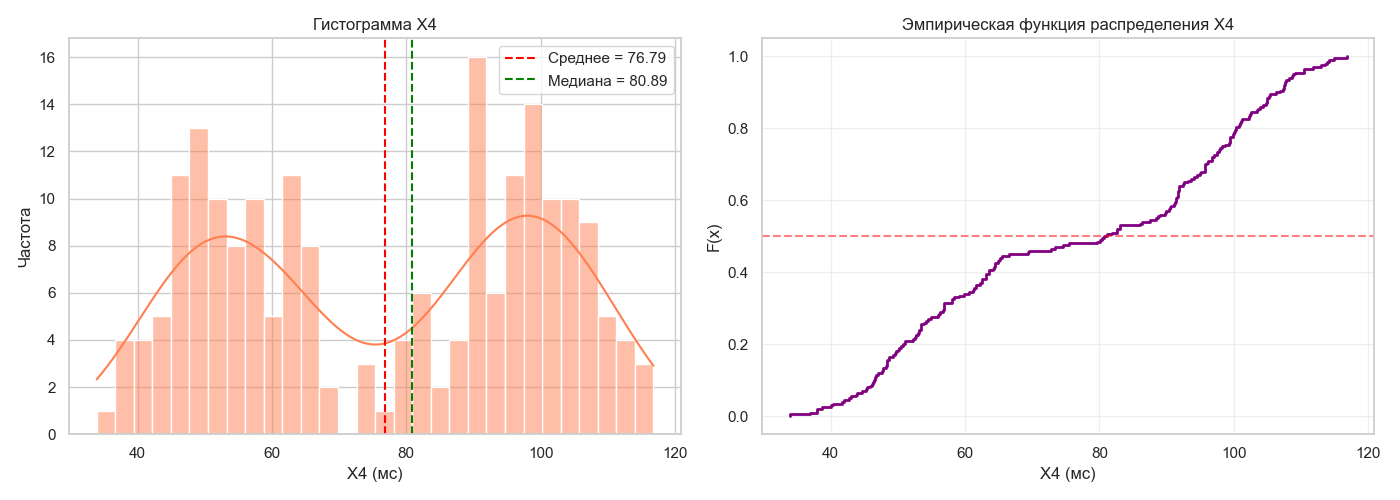
\includegraphics[width=1\linewidth]{pic/plot_2026-04-11 02-52-56_5.png}
    \caption{Гистограмма и ЭФР для $X_4$}
    \label{fig:X4_hist}
\end{figure}

Для переменной $X_4$ наблюдаются следующие особенности:

\begin{itemize}
    \item \textbf{Форма распределения:} ярко выраженная \textbf{бимодальность}. Два пика в интервалах $100$--$110$ и $120$--$130$ разделены провалом в области $110$--$120$. ЭФР имеет два крутых участка роста.
    
    \item \textbf{Признаки неоднородности:} данные распадаются на две обособленные подгруппы с центрами, различающимися на $10$--$15$ единиц. Подгруппы практически не перекрываются. Общее среднее не характеризует ни одну из них.
\end{itemize}

\subsection{Кластеризация методом $k$-средних}

Применён алгоритм $k$-средних с $k = 2$.

\begin{figure}[h]
    \centering
    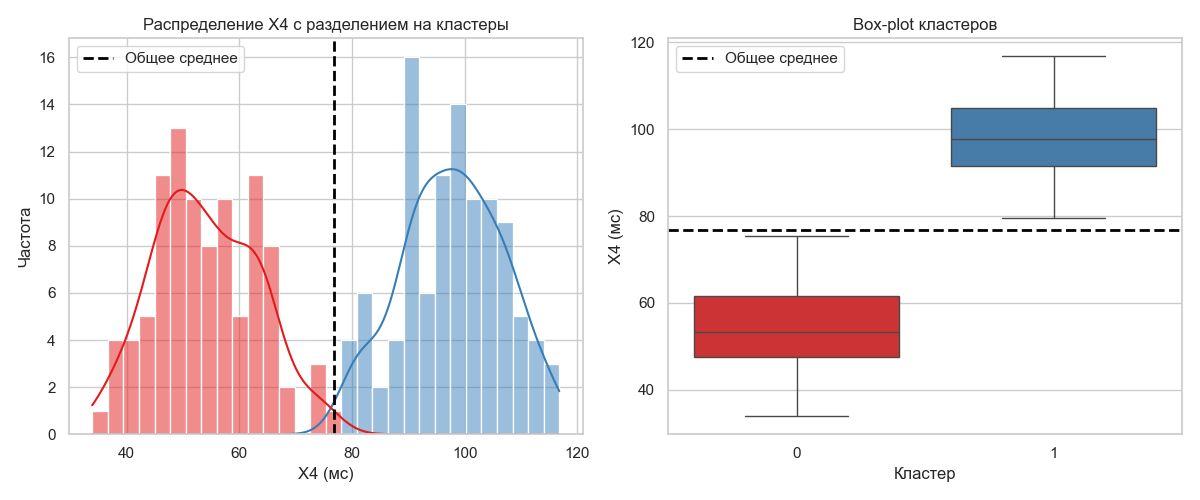
\includegraphics[width=1\linewidth]{pic/plot_2026-04-11 02-52-56_6.png}
    \caption{Распределение $X_4$ по кластерам и box-plot}
    \label{fig:X4_clusters}
\end{figure}

\subsection{Сравнительный анализ}

\begin{table}[h]
\centering
\caption{Характеристики кластеров для $X_4$}
\label{tab:cluster_stats}
\begin{tabular}{cccccc}
\toprule
Кластер & Среднее & Ст. откл. & Кол-во & Минимум & Максимум \\
\midrule
$0$ & $54.02$ & $9.16$ & $96$ & $33.91$ & $75.53$ \\
$1$ & $97.81$ & $8.90$ & $104$ & $79.57$ & $116.79$ \\
\bottomrule
\end{tabular}
\end{table}


\begin{itemize}
    \item \textbf{Различие средних:} $\approx 43.79$ единиц при малых стандартных отклонениях ($\approx 9$). Группы однородны и чётко разделены.
    
    \item \textbf{Диапазоны:} кластеры не перекрываются (максимум $0$: $75.53$, минимум $1$: $79.57$), разрыв $\approx 4$ единицы.
    
    \item \textbf{Объёмы:} кластеры сбалансированы ($96$ и $104$ наблюдения).
\end{itemize}

\subsection{Неинформативность общего среднего}

Общее среднее $\bar{x} \approx 76.79$ попадает в провал между модами и не представляет ни одну из групп. При бимодальной структуре единое среднее маскирует реальное разделение данных. Рекомендуется анализировать подгруппы раздельно или применять кластеризацию.

\section{Итоговый вывод}

\begin{enumerate}
    \item Визуальный анализ (гистограммы по разным правилам и ЭФР) и проверка числовых характеристик позволили определить законы распределения: $X_1 \sim Exp_{\lambda,c}$ (из-за сильной асимметрии), $X_2 \sim U_{a,b}$ (из-за равномерного разброса в границах), $X_3 \sim N_{a,\sigma}$ (колоколообразная форма). Использование разных правил (Скотта, Стерджеса, Фридмана-Диакониса) для гистограмм показало, что правило Фридмана-Диакониса лучше всего улавливает плотность для $X_1$, тогда как правило Стерджеса слишком сглаживает пики.
    
    \item Методы ММ и ММП дали очень близкие оценки параметров, что говорит о высоком качестве и достаточном объёме выборки ($n = 200$).
    
    \item Построенные доверительные интервалы достаточно узки, что гарантирует высокую точность оценок. Точные и асимптотические доверительные интервалы для нормального распределения $X_3$ практически совпали.
    
    \item Анализ $X_4$ подтвердил бимодальную структуру (два режима работы системы). «Общее среднее» (около $76$ мс) попадает в «провал» плотности и не отражает ни одно из реальных состояний системы.
\end{enumerate}